%%%%%%%%%%%%%%%%%%%%%%%%%%%%%%%%%%%%%%%%%%%%%%%%%%%%%%%%%%%%%%%%%
% MUW Presentation
% LaTeX Template
% Version 1.0 (27/12/2016)
%
% License:
% CC BY-NC-SA 4.0 (http://creativecommons.org/licenses/by-nc-sa/3.0/)
%
% Created by:
% Nicolas Ballarini, CeMSIIS, Medical University of Vienna
% nicoballarini@gmail.com
% http://statistics.msi.meduniwien.ac.at/
%
% Customized for UAH by:
% David F. Barrero, Departamento de Automática, UAH
%%%%%%%%%%%%%%%%%%%%%%%%%%%%%%%%%%%%%%%%%%%%%%%%%%%%%%%%%%%%%%%%%

\documentclass[10pt,compress]{beamer} % Change 10pt to make fonts of a different size
\mode<presentation>

\usepackage[spanish]{babel}
\usepackage{fontspec}
\usepackage{tikz}
\usepackage{etoolbox}
\usepackage{xcolor}
\usepackage{xstring}
\usepackage{listings}
\usepackage{multicol}
\usepackage{tabularx}
\usepackage{tikz}
\usetikzlibrary{matrix,chains,positioning,decorations.pathreplacing,arrows,shapes}

\usetheme{UAH}
\usecolortheme{UAH}
\setbeamertemplate{navigation symbols}{} 
\setbeamertemplate{caption}[numbered]

%%%%%%%%%%%%%%%%%%%%%%%%%%%%%%%%%%%%%%%%%%%%%%%%%%%%%%%%%%%%%%%%%
%% Presentation Info
\title[Dataviz]{Data visualization with Matplotlib and Seaborn}
\author{\asignatura\\\carrera}
\institute{}
\date{Departamento de Automática}
%%%%%%%%%%%%%%%%%%%%%%%%%%%%%%%%%%%%%%%%%%%%%%%%%%%%%%%%%%%%%%%%%


%%%%%%%%%%%%%%%%%%%%%%%%%%%%%%%%%%%%%%%%%%%%%%%%%%%%%%%%%%%%%%%%%
%% Descomentar para habilitar barra de navegación superior
\setNavigation
%%%%%%%%%%%%%%%%%%%%%%%%%%%%%%%%%%%%%%%%%%%%%%%%%%%%%%%%%%%%%%%%%

%%%%%%%%%%%%%%%%%%%%%%%%%%%%%%%%%%%%%%%%%%%%%%%%%%%%%%%%%%%%%%%%%
%% Configuración de logotipos en portada
%% Opacidad de los logotipos
\newcommand{\opacidad}{1}
%% Descomentar para habilitar logotipo en pié de página de portada
\renewcommand{\logoUno}{Images/isg.png}
%% Descomentar para habilitar logotipo en pié de página de portada
%\renewcommand{\logoDos}{Images/CCLogo.png}
%% Descomentar para habilitar logotipo en pié de página de portada
%\renewcommand{\logoTres}{Images/ALogo.png}
%% Descomentar para habilitar logotipo en pié de página de portada
%\renewcommand{\logoCuatro}{Images/ELogo.png}
%%%%%%%%%%%%%%%%%%%%%%%%%%%%%%%%%%%%%%%%%%%%%%%%%%%%%%%%%%%%%%%%%

%%%%%%%%%%%%%%%%%%%%%%%%%%%%%%%%%%%%%%%%%%%%%%%%%%%%%%%%%%%%%%%%%
%% FOOTLINE
%% Comment/Uncomment the following blocks to modify the footline
%% content in the body slides. 


%% Option A: Title and institute
\footlineA
%% Option B: Author and institute
%\footlineB
%% Option C: Title, Author and institute
%\footlineC
%%%%%%%%%%%%%%%%%%%%%%%%%%%%%%%%%%%%%%%%%%%%%%%%%%%%%%%%%%%%%%%%%

\begin{document}

%%%%%%%%%%%%%%%%%%%%%%%%%%%%%%%%%%%%%%%%%%%%%%%%%%%%%%%%%%%%%%%%%
% Use this block for a blue title slide with modified footline
{\titlepageBlue
    \begin{frame}
        \titlepage
    \end{frame}
}

\institute{\asignatura}

\begin{frame}[plain]{}
	\begin{block}{Objectives}
		\begin{enumerate}
		\item Motivate the importance of data visualization
		\item Avoid some common mistakes in data visualization
		\item Choose the proper visualization technique
		\item Overview Matplotlib
		\item Introduce Seaborn
		\end{enumerate}
	\end{block}

   \begin{block}{Bibliography}
       Jake VanderPlas. \textit{Python Data Science Handbook}. Chapters 4. O'Reilly. \href{https://jakevdp.github.io/PythonDataScienceHandbook/}{(Link)}.
   \end{block}
\end{frame}

{
\disableNavigation{white}
\begin{frame}[shrink]{Table of Contents}
 \frametitle{Table of Contents}
 %\begin{multicols}{2}
 \tableofcontents
 %\end{multicols}
  % You might wish to add the option [pausesections]
\end{frame}
}

\section{Visualization examples}

\begin{frame}{Visualization examples (I)}
	\begin{columns}
    \column{0.5\textwidth}
		\centering 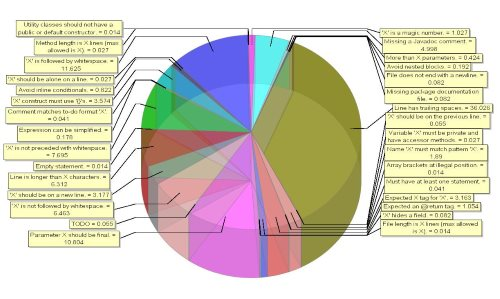
\includegraphics[width=\textwidth]{figs/bad2.jpg}\\
		\centering \tiny \href{http://livingqlikview.com/the-9-worst-data-visualizations-ever-created/}{(Source)}

    \column{0.5\textwidth}
		\centering 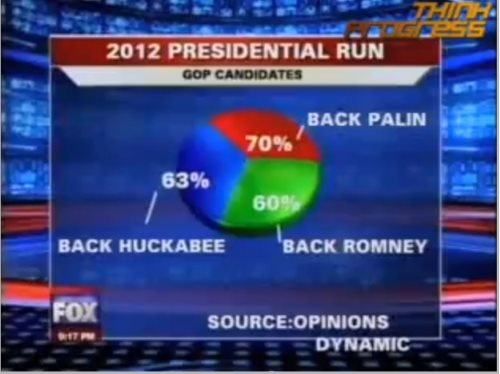
\includegraphics[width=\textwidth]{figs/bad3.jpg}\\
		\centering \tiny \href{http://livingqlikview.com/the-9-worst-data-visualizations-ever-created/}{(Source)}
	\end{columns}
\end{frame}

\begin{frame}{Visualization examples (II)}
	\begin{columns}
    \column{0.5\textwidth}
		\centering 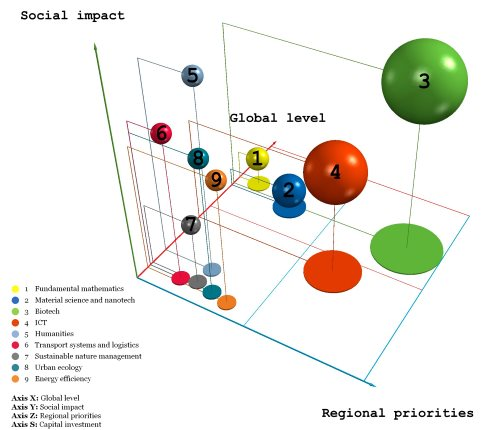
\includegraphics[width=\textwidth]{figs/bad4.jpg}\\
		\centering \tiny \href{http://livingqlikview.com/the-9-worst-data-visualizations-ever-created/}{(Source)}
    \column{0.5\textwidth}
		\centering 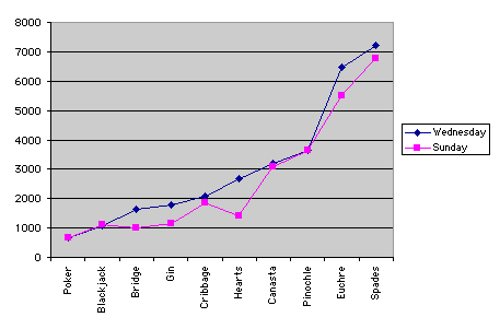
\includegraphics[width=\textwidth]{figs/bad5.jpg}\\
		\centering \tiny \href{http://livingqlikview.com/the-9-worst-data-visualizations-ever-created/}{(Source)}
	\end{columns}
\end{frame}

\begin{frame}{Visualization examples (III)}
	\begin{columns}
    \column{0.5\textwidth}
	\centering 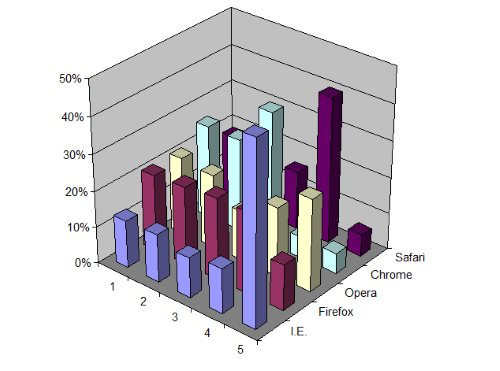
\includegraphics[width=\textwidth]{figs/bad6.jpg}\\
	\centering \tiny \href{http://livingqlikview.com/the-9-worst-data-visualizations-ever-created/}{(Source)}

    \column{0.5\textwidth}
	\centering 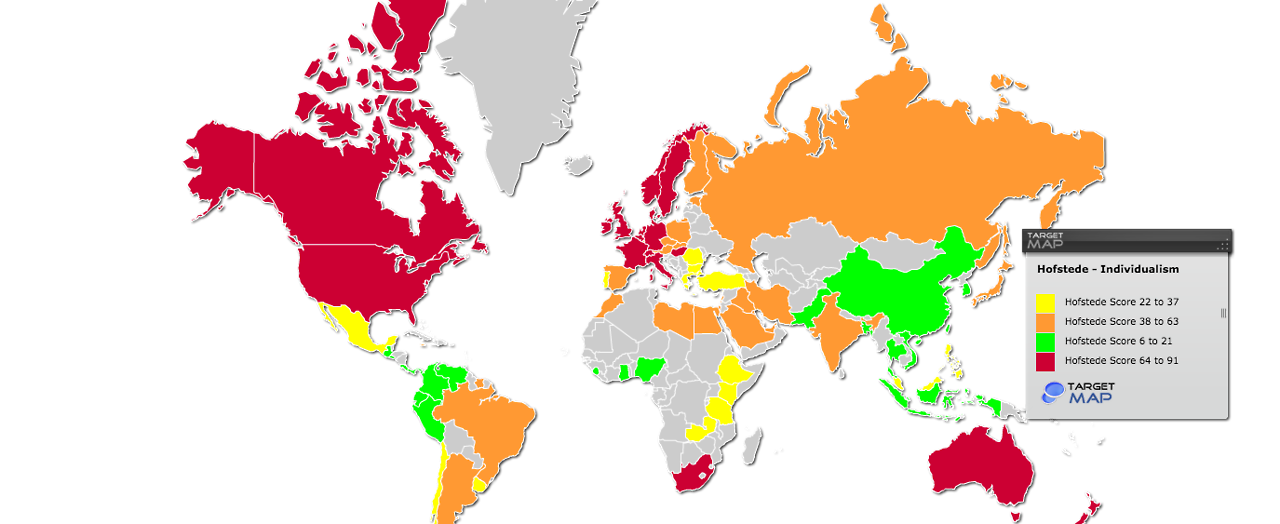
\includegraphics[width=\textwidth]{figs/bad12.png}\\
	\centering \tiny \href{http://viz.wtf/}{(Source)}
	\end{columns}
\end{frame}

\begin{frame}{Visualization examples (IV)}
	\begin{columns}
    \column{0.5\textwidth}
	\centering 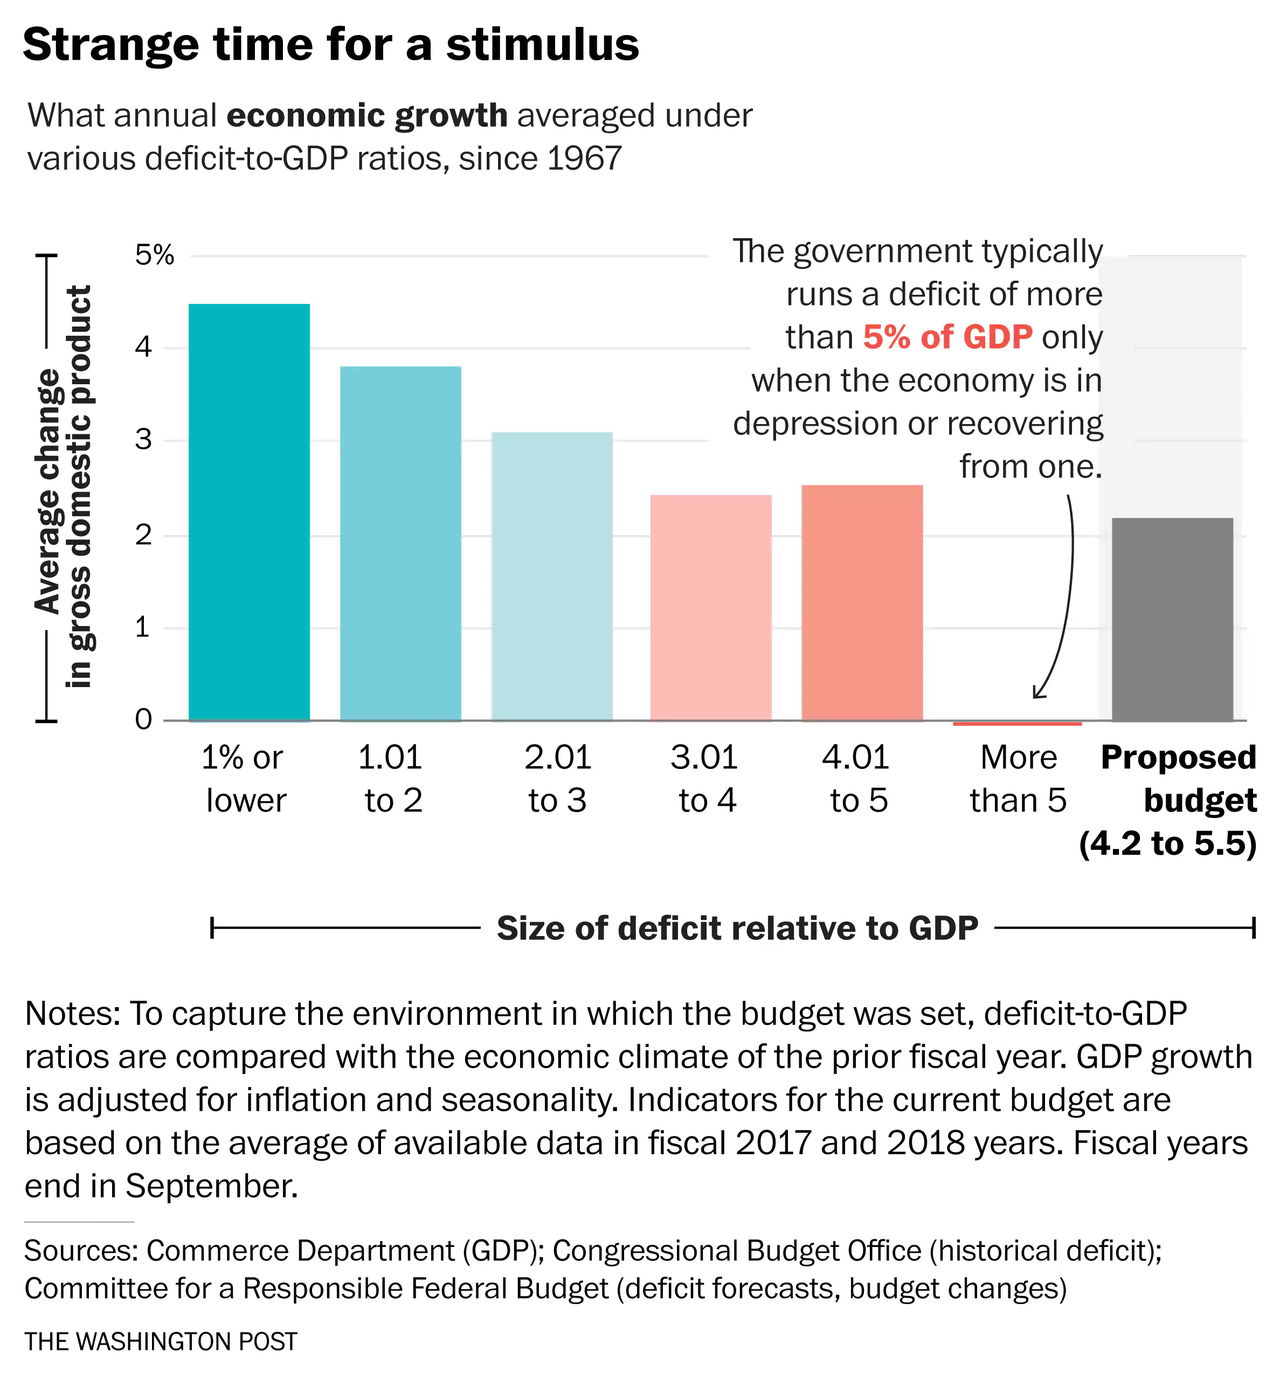
\includegraphics[width=\textwidth]{figs/bad10.png}\\
	\centering \tiny \href{http://viz.wtf/}{(Source)}

    \column{0.5\textwidth}
	\centering 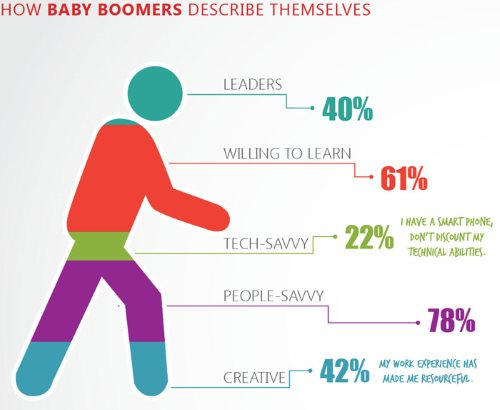
\includegraphics[width=\textwidth]{figs/bad7.jpg}\\
	\centering \tiny \href{http://livingqlikview.com/the-9-worst-data-visualizations-ever-created/}{(Source)}
	\end{columns}
\end{frame}

\begin{frame}{Visualization examples (V)}
	\begin{columns}
    \column{0.7\textwidth}
	\centering 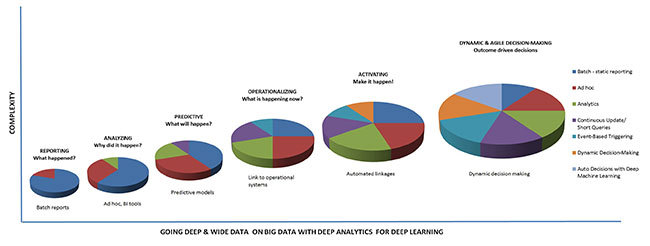
\includegraphics[width=0.8\textwidth]{figs/bad9.jpg}\\
	\centering \tiny \href{http://viz.wtf/}{(Source)}

	\bigskip

	\centering 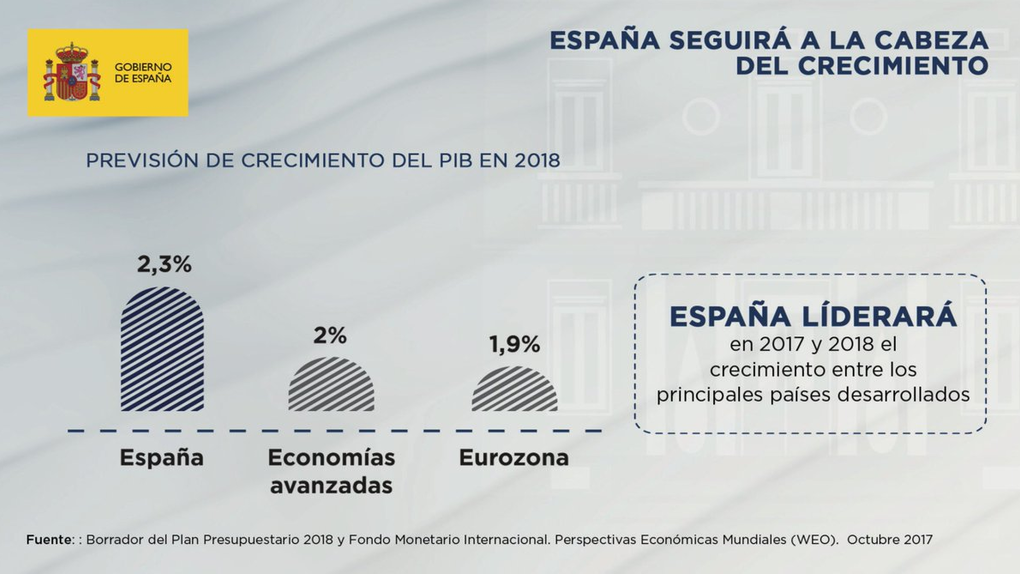
\includegraphics[width=0.8\textwidth]{figs/bad11.png}\\
	\tiny \href{http://viz.wtf/}{(Source)}
	\end{columns}
\end{frame}

\section{Motivation}

\begin{frame}{Motivation (I)}
	Efficient data visualization tips
	\begin{itemize}
		\item \textbf{Define your story}
		\item The chart must tell the story
		\item Don't distract from your story (with irrelevant data or visual elements)
		\item One story, one chart
		\item Put the story comprension in first term
		\item Better several simple charts than one complex chart
		\item Choose colors wisely (color scale or high contrast)
		\item Elements order must support the story (leyend, bars, etc)
		\item There is life beyond pies and bars
		\item Keep it simple, stupid!
	\end{itemize}
\end{frame}

\begin{frame}{Motivation (II)}
	Know your data
	\begin{itemize}
		\item Categorical or numerical
		\item Number of dimensions to represent (1D, 2D, 3D, more dimensions)
	\end{itemize}
	Can you use other representation?
	\begin{itemize}
		\item Chart better than table? ...
		\item ... that depends
	\end{itemize}
	What do you want to represent?
	\begin{itemize}
		\item Distribution, relationship, comparison or composition
	\end{itemize}
	Look for templates: (\url{https://python-graph-gallery.com/})
\end{frame}

\begin{frame}[plain]{Motivation (III)}
	\centering 
\includegraphics[width=0.8\textwidth]{figs/chart-selection-diagram.png}\\
	\centering \tiny \href{https://flex.bi/create-beautiful-dashboard-works/}{(Source)}\\
	\href{http://experception.net/Franconeri_ExperCeptionDotNet_ChartChooser.pdf}{(Alternative resource)}
\end{frame}

\section{Matplotlib}

\begin{frame}[fragile]{Matplotlib (I)}
	\begin{columns}
    \column{0.5\textwidth}
	Matplotlib is a Python package
	\begin{itemize}
		\item Based on NumPy
		\item Imitates Matlab
	\end{itemize}
	Three operation modes
	\begin{itemize}
		\item Scripts. \\Must use \texttt{plt.show()} to enter event loop. Use it once!
		\item IPython shell. \\Must use \texttt{\%matplotlib}
		\item IPython notebook. Two modes
		\begin{itemize}
			\item \texttt{\%matplotlib inline}
			\item \texttt{\%matplotlib notebook}
		\end{itemize}
	\end{itemize}

    \column{0.5\textwidth}
	\begin{block}{\footnotesize{Convention}}
	\vspace{-0.2cm} 
	\begin{lstlisting}
	import matplotlib as mpl
	import matplotlib.pyplot as plt
	\end{lstlisting}
	\vspace{-0.2cm} 
	\end{block}

	\begin{exampleblock}{\footnotesize{myplot.py}}
	\vspace{-0.2cm} 
	\begin{lstlisting}
	import matplotlib.pyplot as plt
	import numpy as np

	x = np.linspace(0, 10, 100)

	plt.plot(x, np.sin(x))
	plt.plot(x, np.cos(x))

	plt.show()
	\end{lstlisting}
	\vspace{-0.2cm} 
	\end{exampleblock}

	\end{columns}
\end{frame}

\begin{frame}[fragile]{Matplotlib (II)}
	Matplotlib comes with two interfaces
	\begin{itemize}
		\item Matlab-like. Old-fashioned function-oriented API.
		\item Object-oriented. Object-oriented and more powerfull API.
	\end{itemize}

	\begin{columns}
    \column{0.5\textwidth}
	\begin{exampleblock}{Matlab API}
	\vspace{-0.2cm} 
	\begin{lstlisting}
	plt.figure()  # create a plot

	# create the first of two panels and set current axis
	plt.subplot(2, 1, 1) # (rows, columns, panel number)
	plt.plot(x, np.sin(x))

	# create the second panel and set current axis
	plt.subplot(2, 1, 2)
	plt.plot(x, np.cos(x));
	\end{lstlisting}
	\vspace{-0.2cm} 
	\end{exampleblock}

    \column{0.5\textwidth}
	\begin{exampleblock}{OO API}
	\vspace{-0.2cm} 
	\begin{lstlisting}
	plt.figure()  # create a plot

	# create the first of two panels and set current axis
	plt.subplot(2, 1, 1) # (rows, columns, panel number)
	plt.plot(x, np.sin(x))

	# create the second panel and set current axis
	plt.subplot(2, 1, 2)
	plt.plot(x, np.cos(x));
	\end{lstlisting}
	\vspace{-0.2cm} 
	\end{exampleblock}
	\end{columns}
\end{frame}

\begin{frame}[fragile]{Matplotlib (III)}
	\begin{columns}
    \column{0.5\textwidth}
		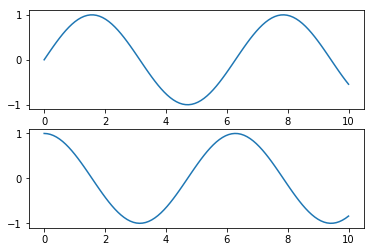
\includegraphics[width=\textwidth]{figs/api.png}
	\end{columns}
\end{frame}

\begin{frame}[fragile]{Matplotlib (IV)}
	\begin{columns}
    \column{0.5\textwidth}
	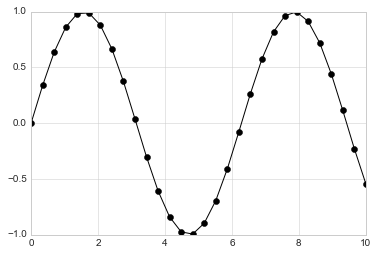
\includegraphics[width=\textwidth]{figs/matplotlib-sin.png}\\

	\begin{exampleblock}{}
	\vspace{-0.2cm} 
	\begin{lstlisting}
	plt.plot(x, np.sin(x), '-ok', color='black')
	\end{lstlisting}
	\vspace{-0.2cm} 
	\end{exampleblock}

    \column{0.5\textwidth}
	\centering 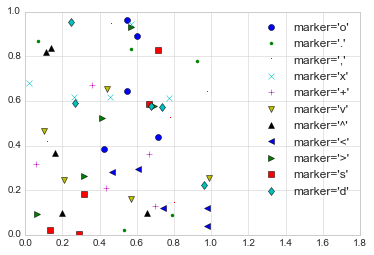
\includegraphics[width=\textwidth]{figs/matplotlib-scatterplot.png}\\
	\begin{exampleblock}{}
	\vspace{-0.2cm} 
	\begin{lstlisting}[basicstyle=\tiny]
	for marker in ['o', '.', ',', 'x', '+', 'v', '^', '<', '>', 's', 'd']:
	    plt.plot(rng.rand(5), rng.rand(5), marker,
	         label="marker='{0}'".format(marker))
	 plt.legend(numpoints=1)
	 plt.xlim(0, 1.8);
	\end{lstlisting}
	\vspace{-0.2cm} 
	\end{exampleblock}
	\end{columns}
\end{frame}

\begin{frame}[fragile]{Matplotlib (V)}
	\begin{columns}
    \column{0.5\textwidth}
	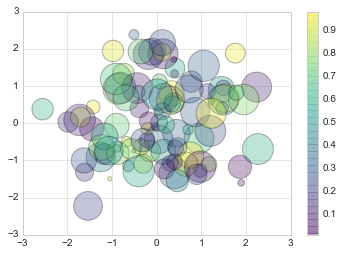
\includegraphics[width=\textwidth]{figs/matplotlib-scatterplot2.png}\\

	\begin{exampleblock}{}
	\vspace{-0.2cm} 
	\begin{lstlisting}[basicstyle=\tiny]
	rng = np.random.RandomState(0)
	x = rng.randn(100)
	y = rng.randn(100)
	colors = rng.rand(100)
	sizes = 1000 * rng.rand(100)

	plt.scatter(x, y, c=colors, s=sizes, alpha=0.3,
	            cmap='viridis')
				plt.colorbar();  # show color scale
	\end{lstlisting}
	\vspace{-0.2cm} 
	\end{exampleblock}

    \column{0.5\textwidth}
	\centering 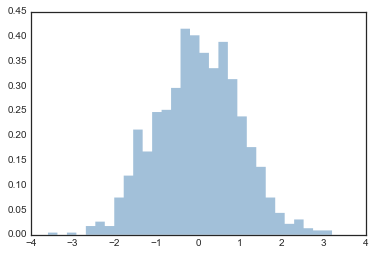
\includegraphics[width=\textwidth]{figs/matplotlib-histogram.png}\\
	\begin{exampleblock}{}
	\vspace{-0.2cm} 
	\begin{lstlisting}[basicstyle=\tiny]
	data = np.random.randn(1000)

	plt.hist(data, bins=30, normed=True, alpha=0.5,
         histtype='stepfilled', color='steelblue',
         edgecolor='none');
	\end{lstlisting}
	\vspace{-0.2cm} 
	\end{exampleblock}
	\end{columns}
\end{frame}

\begin{frame}[fragile]{Matplotlib (VI)}
	\begin{columns}
    \column{0.5\textwidth}
	\begin{exampleblock}{}
	\vspace{-0.2cm} 
	\begin{lstlisting}[basicstyle=\tiny]
	ax = plt.axes(projection='3d')

	# Data for a three-dimensional line
	zline = np.linspace(0, 15, 1000)
	xline = np.sin(zline)
	yline = np.cos(zline)
	ax.plot3D(xline, yline, zline, 'gray')

	# Data for three-dimensional scattered points
	zdata = 15 * np.random.random(100)
	xdata = np.sin(zdata) + 0.1 * np.random.randn(100)
	ydata = np.cos(zdata) + 0.1 * np.random.randn(100)
	ax.scatter3D(xdata, ydata, zdata, c=zdata, cmap='Greens');
	\end{lstlisting}
	\vspace{-0.2cm} 
	\end{exampleblock}

    \column{0.5\textwidth}
	\centering 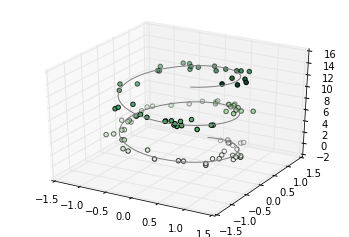
\includegraphics[width=\textwidth]{figs/matplotlib-3d.png}\\
	\end{columns}
\end{frame}

\subsection{Seaborn}

\begin{frame}[fragile]{Seaborn (I)}
	\begin{columns}
    \column{0.65\textwidth}
	Seaborn is a modern data-visualization Python package
	\begin{itemize}
		\item Based on matplotlib
		\item ... it uses matplotlib indeed
		\item Pandas-aware
		\item High level
		\item Advanced visualizations
		\item Easy to use
	\end{itemize}
	Still under development! (v. 0.9)
    \column{0.35\textwidth}
	\begin{block}{\footnotesize{Convention}}
	\vspace{-0.2cm} 
	\begin{lstlisting}
	import seaborn as sns
	\end{lstlisting}
	\vspace{-0.2cm} 
	\end{block}

	\begin{alertblock}{}
	\vspace{-0.2cm} 
	\footnotesize{This documentation is for Seaborn 0.9 or newer}
	\vspace{-0.2cm} 
	\end{alertblock}

	\end{columns}
\end{frame}

\begin{frame}[fragile]{Seaborn (II)}
	\begin{columns}
    \column{0.5\textwidth}
	Display initialization
	\begin{itemize}
		\item \texttt{plt.show()}
		\item \texttt{\%matplotlib}
	\end{itemize}
	Style initialization
	\begin{itemize}
		\item Default Seaborn style \texttt{sns.set()}
		\item By default, same style than matplotlib
	\end{itemize}
	Several functions ...
	\begin{itemize}
		\item ... similar parameters
	\end{itemize}

    \column{0.5\textwidth}
	\begin{block}{Parameters}
	\begin{itemize}
		\item x: Data axis x
		\item y: Data axis Y
		\item data: Dataframe name
		\item hue: Color
		\item style: Style
		\item sizes: Size
		\item kind: Alternate representation
	\end{itemize}
	\end{block}
	\end{columns}
\end{frame}

\begin{frame}[fragile]{Seaborn (III)}
	\begin{columns}
    \column{0.4\textwidth}
		\begin{block}{Typical Seaborn usage}
		\begin{enumerate}
			\item Prepare data
			\item Set up aesthetics
			\item Plot
			\item Customize the plot
		\end{enumerate}
	\end{block}


    \column{0.6\textwidth}
		\begin{exampleblock}{}
			\vspace{-0.2cm} 
			\begin{lstlisting}[basicstyle=\tiny]
			import matplotlib.pyplot as plt
			import seaborn as sns
			# Prepare data
			tips = sns.load_dataset("tips")
			# Set up aesthetics
			sns.set_style("whitegrid")
			# Plot
			g = sns.lmplot(x="tip",y="total_bill", data=tips,aspect=2)
			# Plot customization
			g = (g.set_axis_labels("Tip","Total bill(USD)").set(xlim=(0,10),ylim=(0,100)))
			plt.title("title")
			plt.show(g)
			\end{lstlisting}
			\vspace{-0.2cm} 
		\end{exampleblock}

		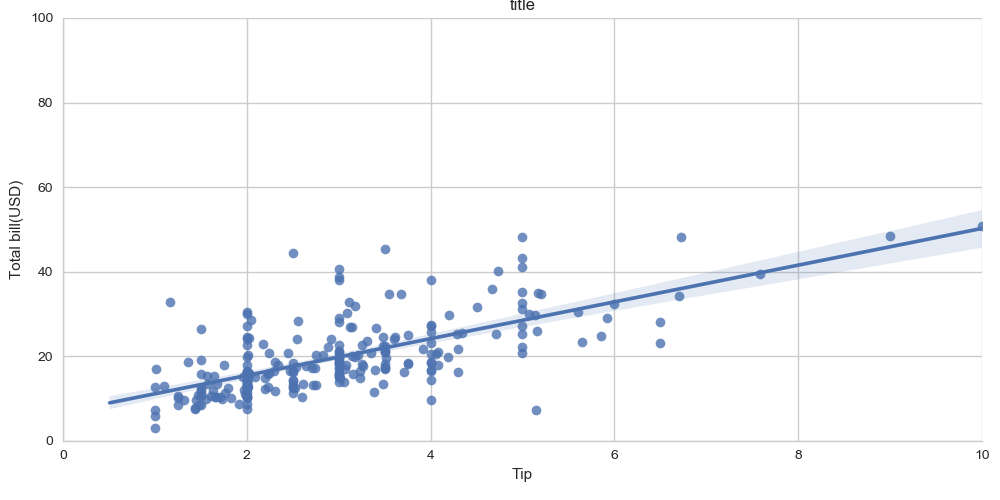
\includegraphics[width=\textwidth]{figs/sns-lm.png}\\
	\end{columns}
\end{frame}

\subsection{Seaborn datasets}

\begin{frame}[fragile]{Seaborn}{Datasets (I)}
	Seaborn comes with several dummy datasets
	\begin{itemize}
		\item \texttt{sns.load\_dataset('name')}
	\end{itemize}
	We will use two datasets
	\begin{itemize}
		\item 'iris': The classical iris dataset, numerical
		\item 'tips': Numeric and categorical variables
	\end{itemize}

	\footnotesize{
	\begin{exampleblock}{\footnotesize{Tips dataset}}
	>>> tips = sns.load\_dataset('tips')\\
	>>> print(tips.head())\\
	\begin{tabular}{lrrllllr}
		\hline
		{} &  total\_bill &   tip &     sex & smoker &  day &    time &  size \\
		\hline
		0 &       16.99 &  1.01 &  Female &     No &  Sun &  Dinner &     2 \\
		1 &       10.34 &  1.66 &    Male &     No &  Sun &  Dinner &     3 \\
		2 &       21.01 &  3.50 &    Male &     No &  Sun &  Dinner &     3 \\
		3 &       23.68 &  3.31 &    Male &     No &  Sun &  Dinner &     2 \\
		4 &       24.59 &  3.61 &  Female &     No &  Sun &  Dinner &     4 \\
		\hline
	\end{tabular}
	\end{exampleblock}
	}
\end{frame}

\begin{frame}[fragile]{Seaborn}{Datasets (II)}
	\footnotesize{
	\begin{exampleblock}{\footnotesize{Iris dataset}}
	>>> iris = sns.load\_dataset('iris')\\
	>>> print(iris.head())\\
	\begin{tabular}{lrrrrl}
	\hline
	{} &  sepal\_length &  sepal\_width &  petal\_length &  petal\_width & species \\
	\hline
	0 &           5.1 &          3.5 &           1.4 &          0.2 &  setosa \\
	1 &           4.9 &          3.0 &           1.4 &          0.2 &  setosa \\
	2 &           4.7 &          3.2 &           1.3 &          0.2 &  setosa \\
	3 &           4.6 &          3.1 &           1.5 &          0.2 &  setosa \\
	4 &           5.0 &          3.6 &           1.4 &          0.2 &  setosa \\
	\hline
	\end{tabular}
	\end{exampleblock}
	}

	\centering 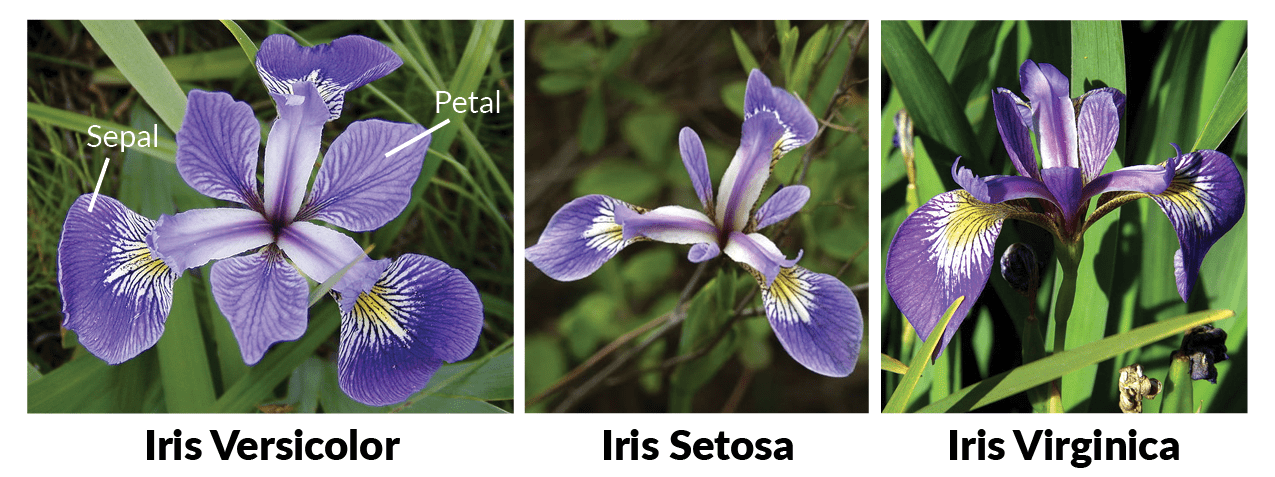
\includegraphics[width=0.7\textwidth]{figs/iris-machinelearning.png}\\
	\centering \href{http://www.lac.inpe.br/~rafael.santos/Docs/R/CAP394/WholeStory-Iris.html}{(Source)}
\end{frame}

\subsection{Distributions}

\begin{frame}[fragile]{Seaborn}{Distributions (I)}
	\begin{columns}[t]
    \column{0.5\textwidth}
	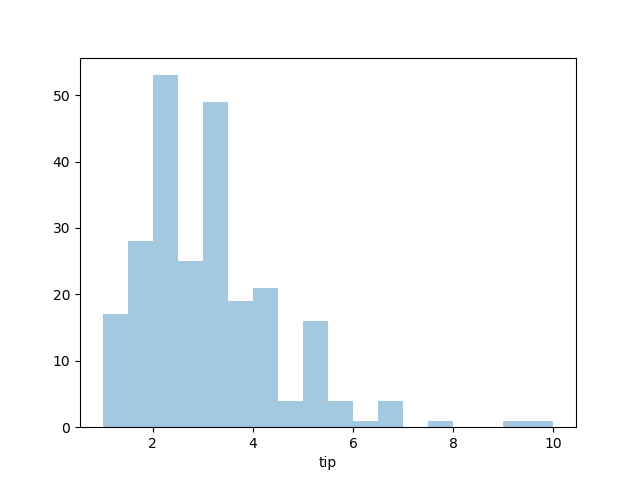
\includegraphics[width=\textwidth]{figs/sns-histogram.png}\\

	\begin{exampleblock}{\footnotesize{Histogram}}
	\vspace{-0.2cm} 
	\begin{lstlisting}[basicstyle=\small]
	sns.distplot(tips['tip'], kde=False)
	\end{lstlisting}
	\vspace{-0.2cm} 
	\end{exampleblock}

    \column{0.5\textwidth}
	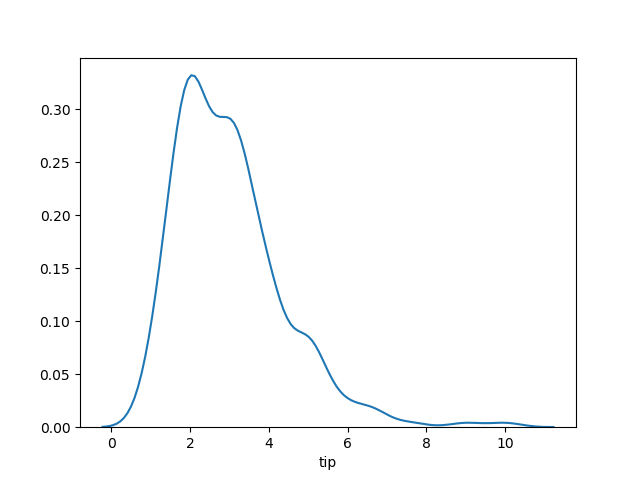
\includegraphics[width=\textwidth]{figs/sns-histogram2.png}\\
	\begin{exampleblock}{\footnotesize{Density plot}}
	\vspace{-0.2cm} 
	\begin{lstlisting}[basicstyle=\small]
	sns.distplot(tips['tip'], hist=False)
	\end{lstlisting}
	\vspace{-0.2cm} 
	\end{exampleblock}
	\end{columns}
\end{frame}

\begin{frame}[fragile]{Seaborn}{Distributions (II)}
	\begin{columns}[t]
    \column{0.5\textwidth}
	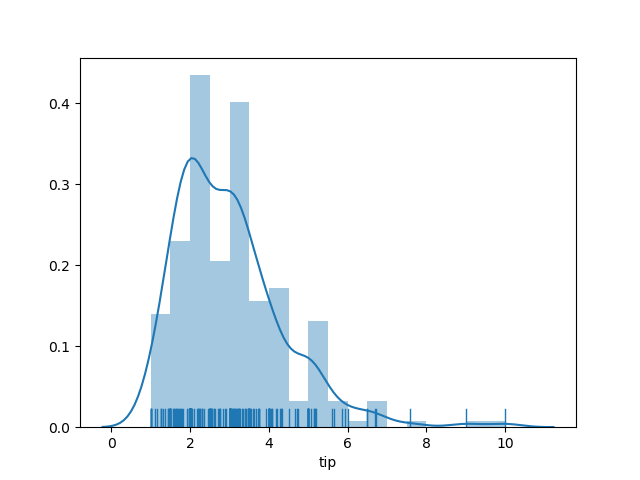
\includegraphics[width=\textwidth]{figs/sns-histogram3.png}\\

	\begin{exampleblock}{\footnotesize{Histogram + density plot}}
	\vspace{-0.2cm} 
	\begin{lstlisting}[basicstyle=\small]
	sns.distplot(tips['tip'], rug=True)
	\end{lstlisting}
	\vspace{-0.2cm} 
	\end{exampleblock}

    \column{0.5\textwidth}
	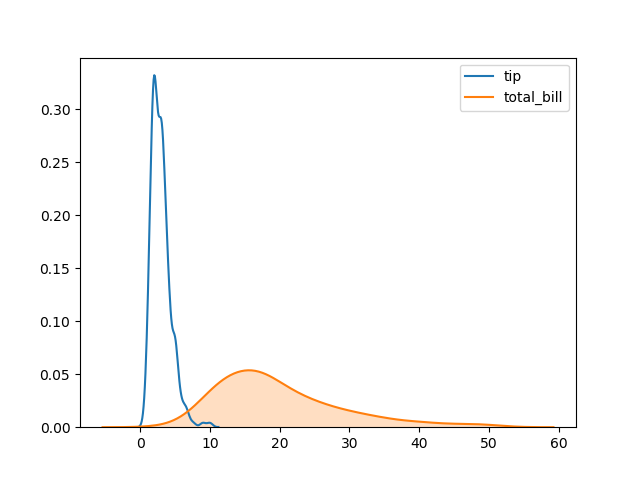
\includegraphics[width=\textwidth]{figs/sns-histogram4.png}\\
	\begin{exampleblock}{\footnotesize{Density plot}}
	\vspace{-0.2cm} 
	\begin{lstlisting}[basicstyle=\small]
	sns.kdeplot(tips['tip'])
	sns.kdeplot(tips['total_bill'], shade=True)
	\end{lstlisting}
	\vspace{-0.2cm} 
	\end{exampleblock}
	\end{columns}
\end{frame}

\begin{frame}[fragile]{Seaborn}{Relationships (I)}
	\centering Scatterplots

	\begin{columns}[t]
    \column{0.33\textwidth}
	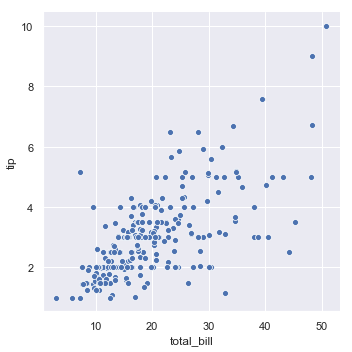
\includegraphics[width=\textwidth]{figs/sns-scatterplot.png}\\
	\begin{exampleblock}{}
	\vspace{-0.2cm} 
	\begin{lstlisting}[basicstyle=\tiny]
	sns.relplot(x="total_bill", y="tip", data=tips)
	\end{lstlisting}
	\vspace{-0.2cm} 
	\end{exampleblock}

    \column{0.33\textwidth}
	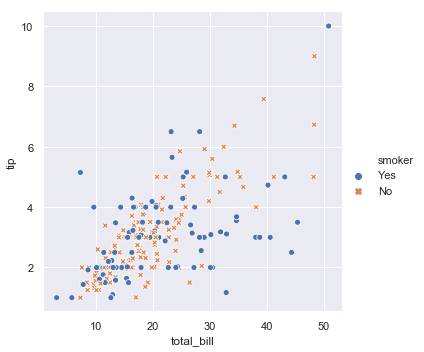
\includegraphics[width=\textwidth]{figs/sns-scatterplot2.png}\\
	\begin{exampleblock}{}
	\vspace{-0.2cm} 
	\begin{lstlisting}[basicstyle=\tiny]
	sns.relplot(x="total_bill", y="tip", hue="smoker", style="smoker", data=tips)
	\end{lstlisting}
	\vspace{-0.2cm} 
	\end{exampleblock}

    \column{0.33\textwidth}
	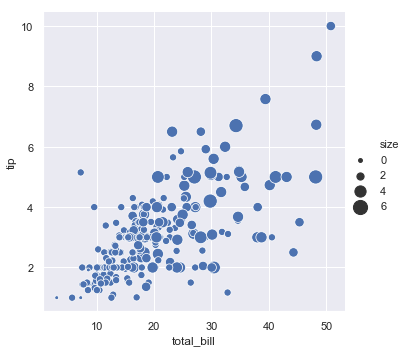
\includegraphics[width=\textwidth]{figs/sns-scatterplot3.png}\\
	\begin{exampleblock}{}
	\vspace{-0.2cm} 
	\begin{lstlisting}[basicstyle=\tiny]
	sns.relplot(x="total_bill", y="tip", size="size", sizes=(15, 200), data=tips);
	\end{lstlisting}
	\vspace{-0.2cm} 
	\end{exampleblock}

	\end{columns}

	Seaborn >= 0.9
\end{frame}

\begin{frame}[fragile]{Seaborn}{Relationships (II)}
	\begin{columns}[t]
    \column{0.5\textwidth}
	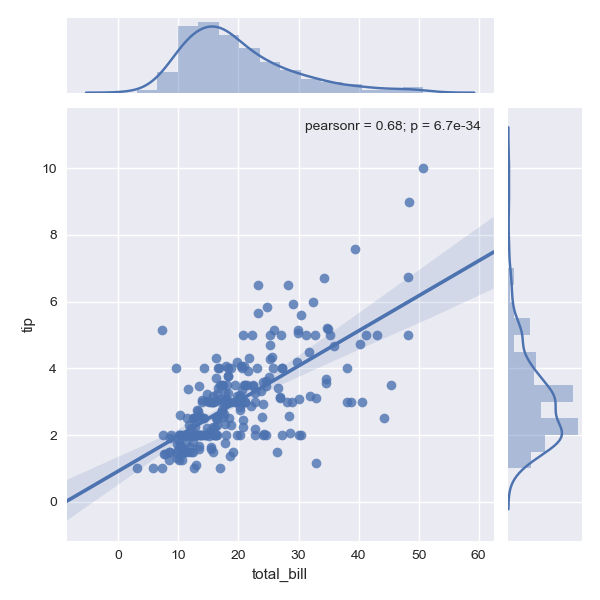
\includegraphics[width=\textwidth]{figs/sns-jointplot.png}\\
	\begin{exampleblock}{}
	\vspace{-0.2cm} 
	\begin{lstlisting}[basicstyle=\tiny]
	sns.jointplot("total_bill", "tip", tips, kind="reg")
	\end{lstlisting}
	\vspace{-0.2cm} 
	\end{exampleblock}

 	 \column{0.5\textwidth}
	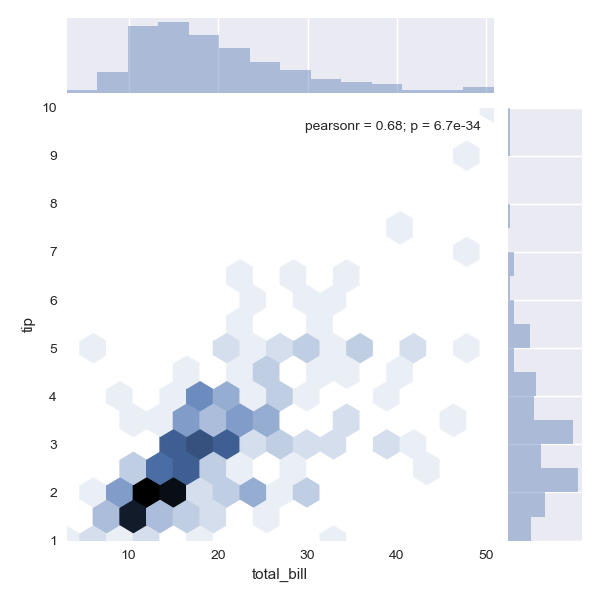
\includegraphics[width=\textwidth]{figs/sns-jointplothex.png}\\
	\begin{exampleblock}{}
	\vspace{-0.2cm} 
	\begin{lstlisting}[basicstyle=\tiny]
	sns.jointplot("total_bill", "tip", tips , kind="hex")
	\end{lstlisting}
	\vspace{-0.2cm} 
	\end{exampleblock}

	\end{columns}
\end{frame}

\begin{frame}[fragile]{Seaborn}{Relationships (III)}
	\begin{columns}
    \column{0.5\textwidth}
	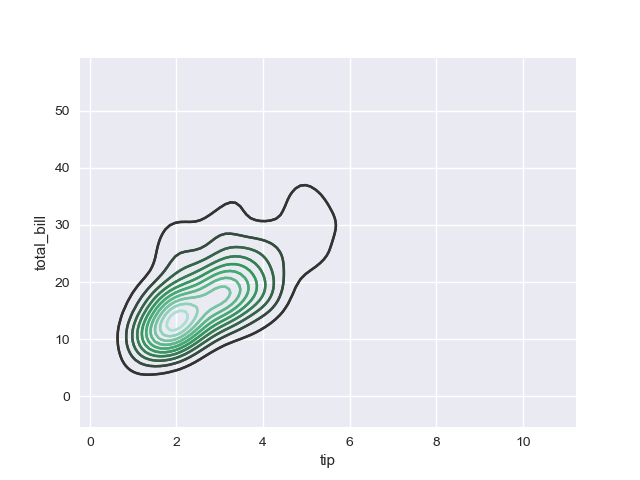
\includegraphics[width=\textwidth]{figs/sns-kdeplot.png}\\
	\begin{exampleblock}{}
	\vspace{-0.2cm} 
	\begin{lstlisting}[basicstyle=\tiny]
	sns.kdeplot(tips['tip'], tips['total_bill'])
	\end{lstlisting}
	\vspace{-0.2cm} 
	\end{exampleblock}

 	 \column{0.5\textwidth}
	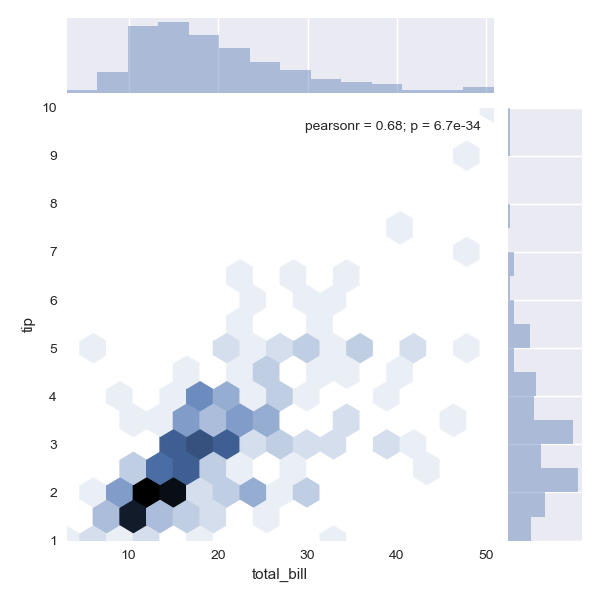
\includegraphics[width=\textwidth]{figs/sns-jointplothex.png}\\
	\begin{exampleblock}{}
	\vspace{-0.2cm} 
	\begin{lstlisting}[basicstyle=\tiny]
	sns.jointplot("total_bill", "tip", tips , kind="hex")
	\end{lstlisting}
	\vspace{-0.2cm} 
	\end{exampleblock}

	\end{columns}
\end{frame}

\begin{frame}[fragile]{Seaborn}{Relationships (IV)}
	\begin{columns}
    \column{0.5\textwidth}
	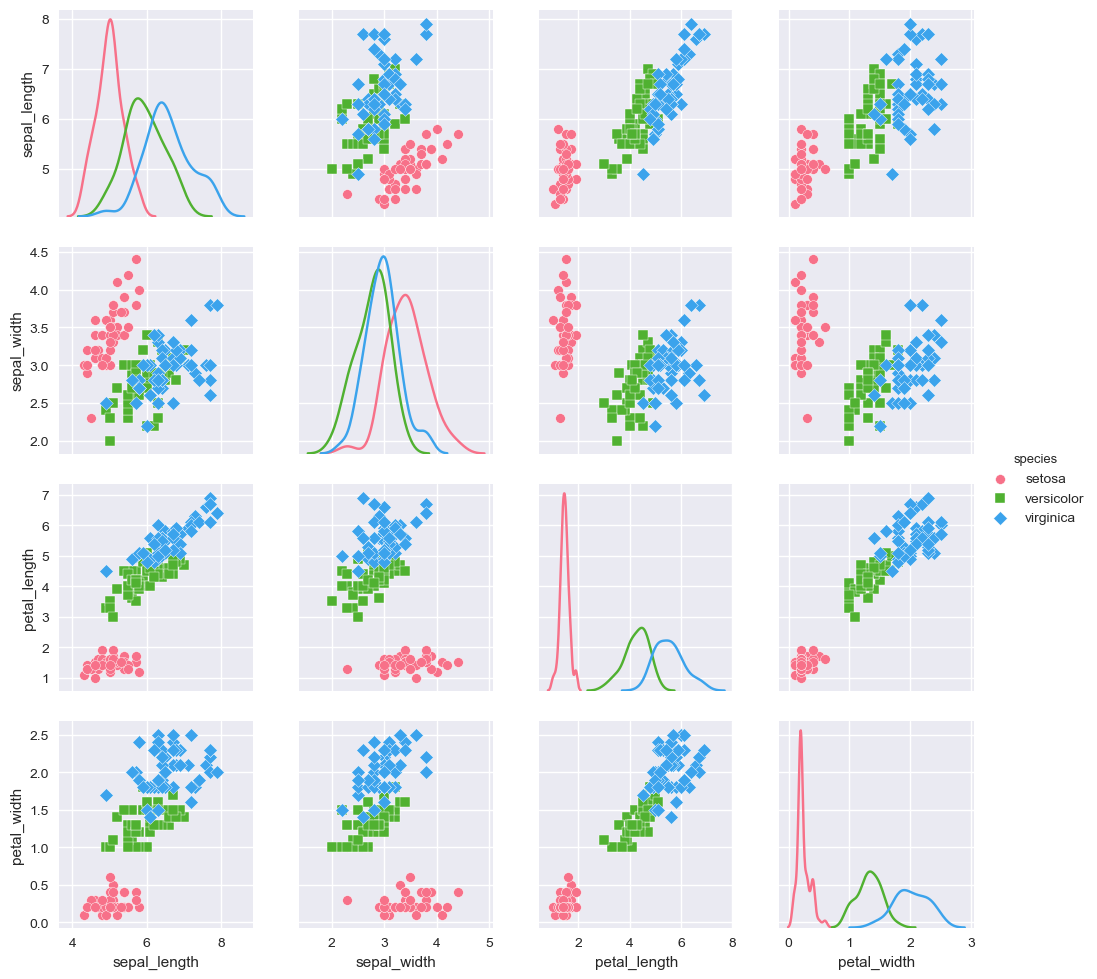
\includegraphics[width=\textwidth]{figs/sns-pairkde.png}\\
	\begin{exampleblock}{\footnotesize{Scatterplot matrix}}
	\vspace{-0.2cm} 
	\begin{lstlisting}[basicstyle=\tiny]
	sns.pairplot(iris, hue="species", palette="husl", markers=["o", "s", "D"], diag_kind='kde')
	\end{lstlisting}
	\vspace{-0.2cm} 
	\end{exampleblock}

    \column{0.5\textwidth}
	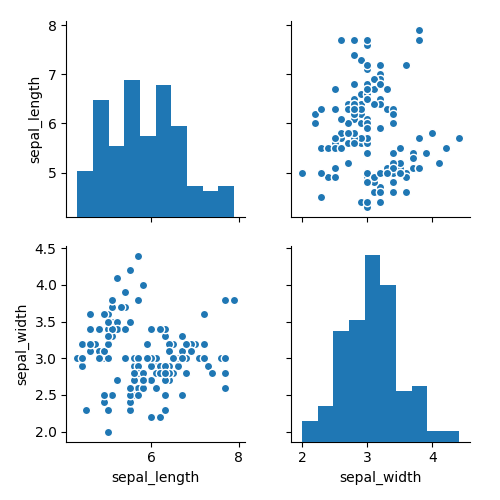
\includegraphics[width=\textwidth]{figs/sns-pair.png}\\
	\begin{exampleblock}{\footnotesize{Scatterplot matrix}}
	\vspace{-0.2cm} 
	\begin{lstlisting}[basicstyle=\tiny]
	sns.pairplot(iris, vars=["sepal_length", "sepal_width"])
	\end{lstlisting}
	\vspace{-0.2cm} 
	\end{exampleblock}

	\end{columns}
\end{frame}

\begin{frame}[fragile]{Seaborn}{Comparisons (I)}
	\begin{columns}
    \column{0.5\textwidth}
	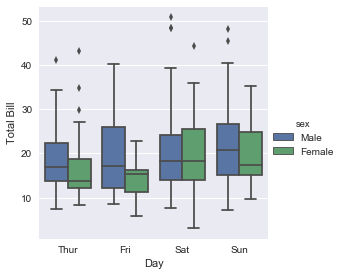
\includegraphics[width=\textwidth]{figs/sns-boxplot.png}\\
	\begin{exampleblock}{\footnotesize{Boxplot}}
	\vspace{-0.2cm} 
	\begin{lstlisting}[basicstyle=\tiny]
	with sns.axes_style(style='ticks'):
	    g = sns.factorplot("day", "total_bill", "sex", data=tips, kind="box")
		g.set_axis_labels("Day", "Total Bill")
	\end{lstlisting}
	\vspace{-0.2cm} 
	\end{exampleblock}

 	 \column{0.5\textwidth}
	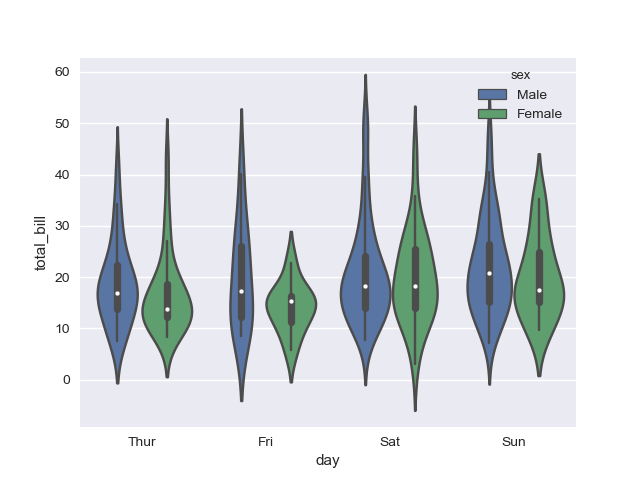
\includegraphics[width=\textwidth]{figs/sns-violin.png}\\
	\begin{exampleblock}{\footnotesize{Violin plot}}
	\vspace{-0.2cm} 
	\begin{lstlisting}[basicstyle=\tiny]
	sns.violinplot("day", "total_bill", "sex", data=tips)
	\end{lstlisting}
	\vspace{-0.2cm} 
	\end{exampleblock}

	\end{columns}
\end{frame}

\begin{frame}[fragile]{Seaborn}{Comparisons (II)}
	\begin{columns}
    \column{0.5\textwidth}
	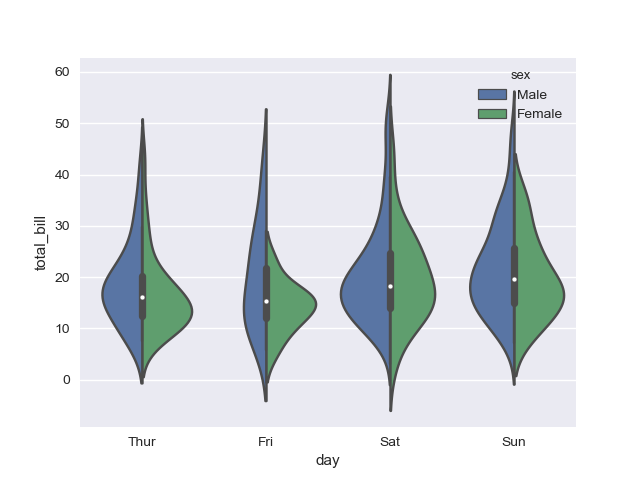
\includegraphics[width=\textwidth]{figs/sns-violin2.png}\\
	\begin{exampleblock}{\footnotesize{Violin plot}}
	\vspace{-0.2cm} 
	\begin{lstlisting}[basicstyle=\tiny]
	sns.violinplot(x="day", y="total_bill", hue="sex", data=tips, split=True)
	\end{lstlisting}
	\vspace{-0.2cm} 
	\end{exampleblock}

 	 \column{0.5\textwidth}
	\centering 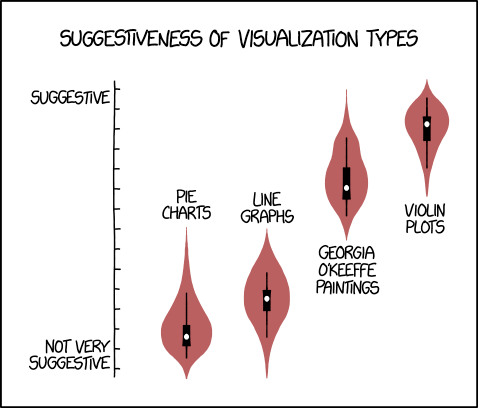
\includegraphics[width=0.7\textwidth]{figs/violin_plots.png}\\
	\tiny \centering \href{https://xkcd.com/1967/}{(Source)}
	\end{columns}
\end{frame}

\begin{frame}[fragile]{Seaborn}{Barplots}
	\begin{columns}
    \column{0.5\textwidth}
	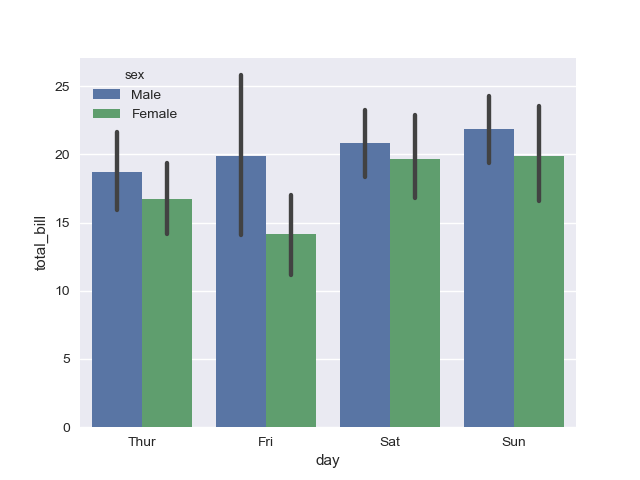
\includegraphics[width=\textwidth]{figs/sns-barplot.png}\\
	\begin{exampleblock}{\footnotesize{Barplot}}
	\vspace{-0.2cm} 
	\begin{lstlisting}[basicstyle=\tiny]
	sns.barplot(x="day", y="total_bill", hue="sex", data=tips)
	\end{lstlisting}
	\vspace{-0.2cm} 
	\end{exampleblock}

    \column{0.5\textwidth}
	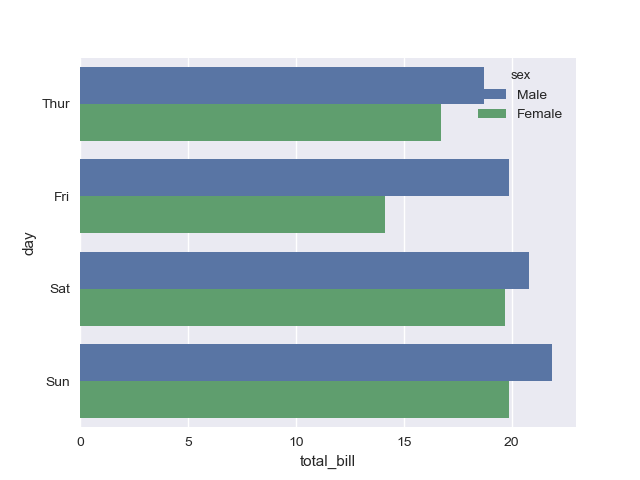
\includegraphics[width=\textwidth]{figs/sns-barplot2.png}\\
	\begin{exampleblock}{\footnotesize{Barplot}}
	\vspace{-0.2cm} 
	\begin{lstlisting}[basicstyle=\tiny]
	sns.barplot(x="total_bill", y="day", hue="sex", data=tips, ci=None)
	\end{lstlisting}
	\vspace{-0.2cm} 
	\end{exampleblock}
	\end{columns}
\end{frame}

\begin{frame}[fragile]{Seaborn}{Continuity}
	\begin{columns}
    \column{0.5\textwidth}
		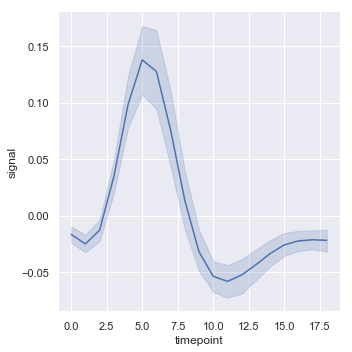
\includegraphics[width=0.9\textwidth]{figs/sns-line.png}\\
		\begin{exampleblock}{\footnotesize{}}
		\vspace{-0.2cm} 
		\begin{lstlisting}[basicstyle=\tiny]
		fmri = sns.load_dataset("fmri")
		sns.relplot(x="timepoint", y="signal", kind="line", data=fmri)
		\end{lstlisting}
		\vspace{-0.2cm} 
		\end{exampleblock}

 	\column{0.5\textwidth}
		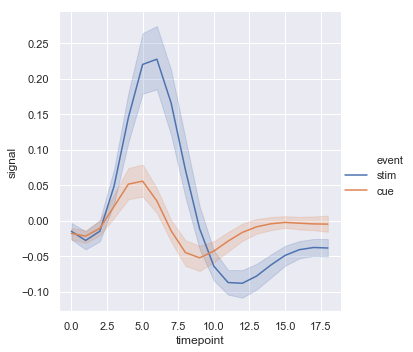
\includegraphics[width=\textwidth]{figs/sns-line2.png}\\
		\begin{exampleblock}{\footnotesize{}}
		\vspace{-0.2cm} 
		\begin{lstlisting}[basicstyle=\tiny]
		sns.relplot(x="timepoint", y="signal", hue="event", kind="line", data=fmri)
		\end{lstlisting}
		\vspace{-0.2cm} 
		\end{exampleblock}
	\end{columns}
	Seaborn >= 0.9
\end{frame}

\begin{frame}[fragile]{Seaborn}{\texttt{FacetGrid}}
	\begin{columns}
    \column{0.5\textwidth}
		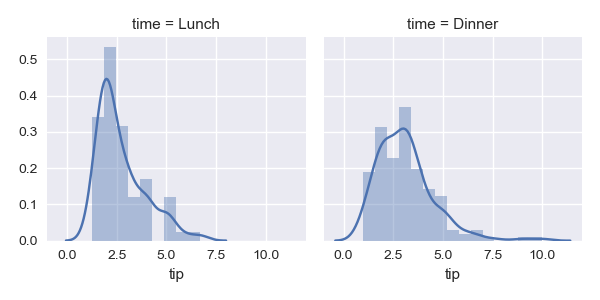
\includegraphics[width=0.9\textwidth]{figs/sns-facethist.png}\\
		\begin{exampleblock}{\footnotesize{}}
		\vspace{-0.2cm} 
		\begin{lstlisting}[basicstyle=\tiny]
		fmri = sns.load_dataset("fmri")
		sns.relplot(x="timepoint", y="signal", kind="line", data=fmri)
		\end{lstlisting}
		\vspace{-0.2cm} 
		\end{exampleblock}

		Seaborn >= 0.9

 	\column{0.5\textwidth}
		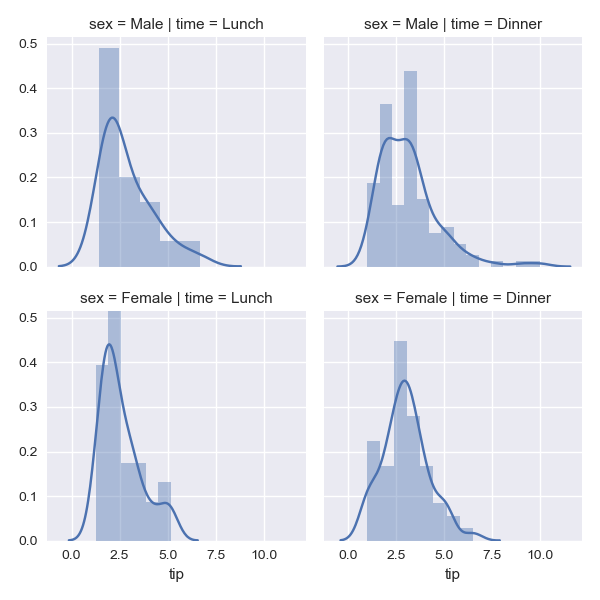
\includegraphics[width=\textwidth]{figs/sns-facethist2.png}\\
		\begin{exampleblock}{\footnotesize{}}
		\vspace{-0.2cm} 
		\begin{lstlisting}[basicstyle=\tiny]
		g = sns.FacetGrid(tips, col="time", row="sex")
		g.map(sns.distplot, "tip")
		\end{lstlisting}
		\vspace{-0.2cm} 
		\end{exampleblock}
	\end{columns}
\end{frame}

\begin{frame}[plain]
	\begin{center}
		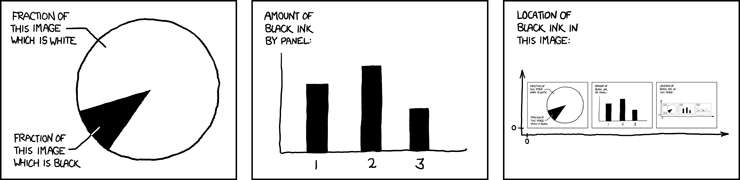
\includegraphics[width=\textwidth]{figs/self_description.png}\\
		\tiny \href{https://xkcd.com/688/}{(Source)}
	\end{center}
\end{frame}

%\begin{frame}[plain]{Solved exercise. Serializando objetos \texttt{Parcela}}{}
%	\vspace{-0.4cm}
  %  \begin{columns}
 %	   \column{0.8\textwidth}
%			\begin{block}{\footnotesize{tasaparcela\_pickle.py}}
%			\vspace{-0.2cm} 
%				\lstinputlisting[basicstyle=\ttfamily\scriptsize]{code/tasaparcela_pickle.py} % contar elementos
%			\vspace{-0.2cm} 
%			\end{block}
%	\end{columns}
	
%\end{frame}


\end{document}
